

\tikzset{every picture/.style={line width=0.75pt}} %set default line width to 0.75pt        
\begin{center}
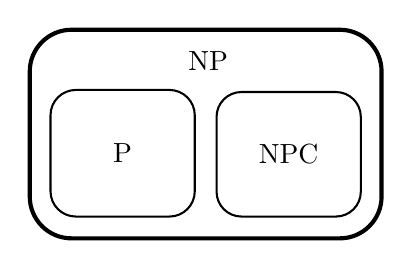
\begin{tikzpicture}[x=0.75pt,y=0.75pt,yscale=-1,xscale=1]
%uncomment if require: \path (0,300); %set diagram left start at 0, and has height of 300

%Rounded Rect [id:dp4469509270957106] 
\draw  [line width=1.5]  (180.5,110.1) .. controls (180.5,99) and (189.5,90) .. (200.6,90) -- (329.9,90) .. controls (341,90) and (350,99) .. (350,110.1) -- (350,170.4) .. controls (350,181.5) and (341,190.5) .. (329.9,190.5) -- (200.6,190.5) .. controls (189.5,190.5) and (180.5,181.5) .. (180.5,170.4) -- cycle ;
%Rounded Rect [id:dp019097988645257136] 
\draw   (190.5,131.2) .. controls (190.5,124.46) and (195.96,119) .. (202.7,119) -- (247.8,119) .. controls (254.54,119) and (260,124.46) .. (260,131.2) -- (260,167.8) .. controls (260,174.54) and (254.54,180) .. (247.8,180) -- (202.7,180) .. controls (195.96,180) and (190.5,174.54) .. (190.5,167.8) -- cycle ;
%Rounded Rect [id:dp3526831805757056] 
\draw   (270.5,132) .. controls (270.5,125.37) and (275.87,120) .. (282.5,120) -- (328,120) .. controls (334.63,120) and (340,125.37) .. (340,132) -- (340,168) .. controls (340,174.63) and (334.63,180) .. (328,180) -- (282.5,180) .. controls (275.87,180) and (270.5,174.63) .. (270.5,168) -- cycle ;

% Text Node
\draw (266.5,105) node  [align=left] {NP};
% Text Node
\draw (225.25,149.5) node  [align=left] {P};
% Text Node
\draw (305.25,150) node  [align=left] {NPC};


\end{tikzpicture}
\end{center}